% !TeX spellcheck = de_DE

\chapter{Hauptteil 1}
Für weitere Entwicklungen wird der Aufbau wie in Bild \ref{fig:sim3} verwendet. Bild \ref{fig:vorgehe} beschreibt die notwendigen Funktionsblöcke. Zuerst wird der Simulator \textit{AirSim} eingerichtet. Weitere Entwicklungen finden jeweils in einem eigenen Container statt, um sie anschließend auf den Bordcomputer verwenden zu können. Die \gls{mav}-Nachrichten werden \acrshort{ros}-Knotenpunkt weiter verbreitet. Mit diesen und dem Bildern aus dem Simulator wird die Hinderniserkennung betrieben. Die generierte Tiefenkarte wird vom \textit{Obstacle Avoidance} Modul verarbeitet. Die so generierten Navigationsinformationen werden dem Flugcontroller wieder zugeführt

\begin{figure}[!h]
	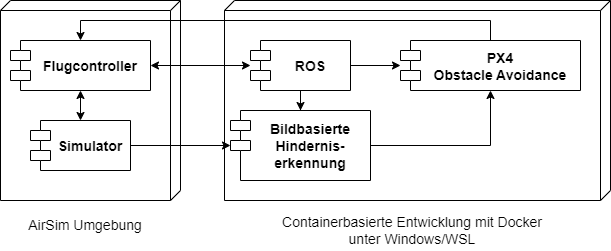
\includegraphics[width=0.7\linewidth]{images/vorgehen_eigenteil.drawio.png}
	\caption{Aufgliederung Bestandteile der Softwareentwicklung}
	\label{fig:vorgehe}
	\end{figure}
%, vorerst ohne Ultraschallsensoren.

\section{Einrichtung der Software}
Der erste Schritt ist das Verbinden des Flugcontrollers mit der \gls{gcs} und das Durchführen eines Updates der Software des Flugcontrollers. Für das Projekt läuft nun PX4, Version $1.13.2$. Anschließend wird die \gls{gcs} keine automatische Verbindung (\textit{AutoConnect}) zu \textit{Pixhawk} Geräten durchzuführen, um die Kabelverbindung für die Simulationssoftware frei zu halten.

Um den Flugcontroller mit AirSim zu verwenden, muss dieser in den \gls{hil}-Modus versetzt werden. Ausführliche Anleitungen sind verfügbar unter \footnote{\url{https://microsoft.github.io/AirSim/px4_setup/\#setting-up-px4-hardware-in-loop}\cite{microsoftcorporationWelcomeAirSim2023}}. Bild \ref{app_sim} zeigt die virtuelle Drohne im Simulator. Anschließend wird der Flugcontroller erneut konfiguriert, über den TELEM2-Port \gls{mav}-Nachrichten zu verbreiten. Nun kann QGroundControl auf zwei Arten betrieben werden:
\begin{compactitem}
    \item Wenn der Simulator gestartet ist, verbreitet er über UDP-Protokoll \gls{mav}-Nachrichten
    \item Per Netzwerkzugriff über den \gls{rpi} auf den Flugcontroller zugreifen. (selbe Variante wird später verwendet, um die \gls{mav}-Nachrichten an \acrshort{ros} weiterzuleiten)
\end{compactitem}

Die Problematik \acrshort{ros} kann hier nur kurz angschnitten werden. Das wichtigste ist in Tabelle \ref{tab:cmp_ros} aufgeführt. Außerdem ist \acrshort{ros} stark an Linux Ubuntu geknüpft und läuft kaum auf anderen Betriebssystemen. Das Vorgängerprojekt sah vor, \acrshort{ros}2 zu verwenden\cite[Kapitel 6.6]{wirthErweiterungBestehendenDrohne2022a}. In \cite{dronecodestiftungObstacleDetectionAvoidance2023} wird Linux Ubuntu 20.04 in Verbindung mit \textit{\acrshort{ros} Noetic} (Version 1) verwendet. Um kompatibel zum Zielsystem zu bleiben wird für das weitere Vorgehen vorerst ein solcher Container mit \textit{\acrshort{ros} Noetic} (Version 1) gesucht. Im DockerHub\footnote{\url{https://hub.docker.com/_/ros/}\cite{dronecodestiftungRosOfficialImage}} stehen diverse Images zur Verfügung. Aufgrund weiterer Vorhaben im Bereich Bildverarbeitung wird das Image \enquote{noetic-perception-focal} verwendet.
\begin{table}[h]
    \begin{minipage}{\linewidth}
    \caption{Vergleich \acrshort{ros} und \acrshort{ros}2}
    \centering
    \label{tab:cmp_ros}
    \begin{tabularx}{\textwidth}{X | X}
        \acrshort{ros} & \acrshort{ros}2 \\
        \hline
        Nicht mehr Weiterentwickelt & Aktive Entwicklung\\
        Verfügbar auf 64-bit PC, 32- und 64-bit ARM & Nur auf 64-bit PC und ARM verfügbar\\
    \end{tabularx}
\end{minipage}
\end{table}

\begin{figure}[h!]
    \centering
    \subfloat[Ausgangszustand Simulator]{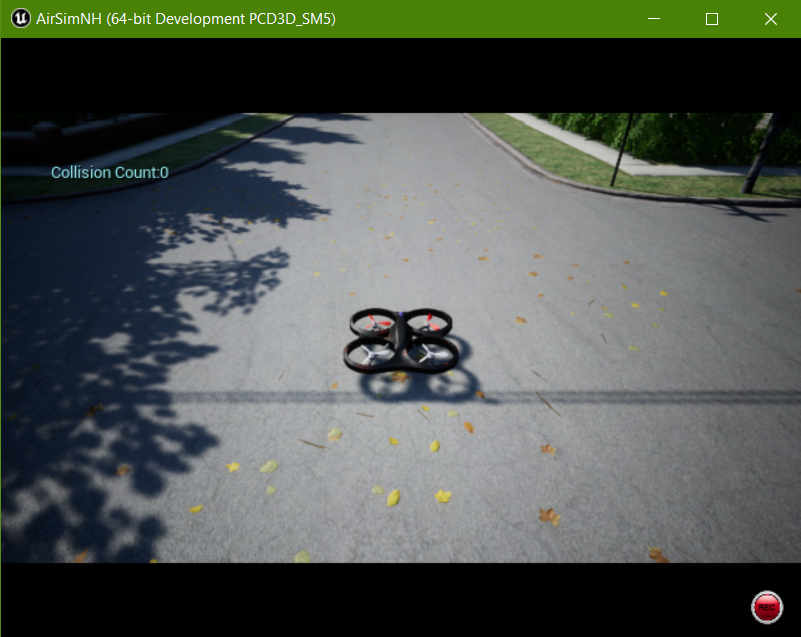
\includegraphics[width=0.5\textwidth]{images/sim_initial.png}}
    \subfloat[Endzustand Simulator nach \textit{offboard\_control}]{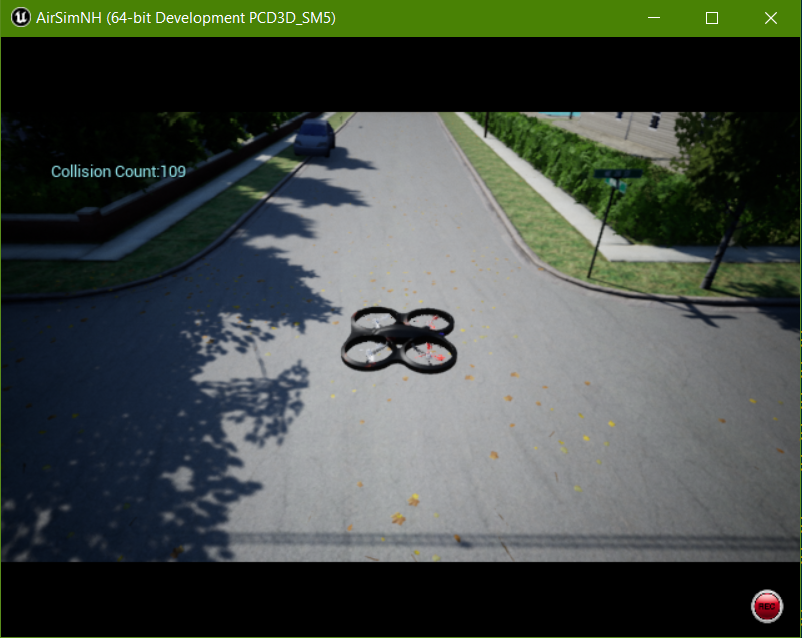
\includegraphics[width=0.5\textwidth]{images/sim_offboard.png} \label{fig:app_sim_ende} (siehe nächstes Kapitel)}
    \caption{Simulation der Drohne unter Windows}
    \label{fig:app_sim}
\end{figure}

\section{Verarbeitung von MAVLink-Nachrichten}
In diesem Kapitel wird der Funktionsblock \enquote{ROS} aus dem Bild \ref{fig:vorgehe} entwickelt. Um \acrshort{ros} laufen zu lassen, sind mehrere Bestandteile notwendig. Nach gängiger Praxis wird für jede Funktion ein eigener Container angelegt. Alle Container verwenden dasselbe Image, sodass dieses nur einmalig gebaut wird und anschließend jeden Container mit eigenem Kommando startet. Diese sind in den folgenden Paragraphen aufgegliedert. Die vollständige Zusammenstellung besteht aus:
\begin{compactitem}
    \item roscore: \acrshort{ros}-Umgebung
    \item rqt: \acrshort{ros}-Überwachung
    \item mavros: \gls{mav}-zu-\acrshort{ros}-Übersetzung
    \item offboard\_control: Beispielanwendung
\end{compactitem}

Alle Container werden mit dem Netzwerk des Host-Computers verknüpft, so müssen keine Ports manuell freigegeben werden.

\subsubsection{roscore}
Um auf die Funktionalität von \acrshort{ros} zugreifen zu können, muss das Programm \enquote{roscore} ähnlich einem Server laufen. Dieses ist in jeder \acrshort{ros}-Umgebung enthalten und wird einmalig gestartet.

\subsubsection{rqt}
Mit dem Tool \enquote{rqt} können \acrshort{ros}-Nachrichten mitgelesen werden. In diesem Anwendungsfall wird das korrekte Ausführen der \acrshort{ros}-Container manuell überwacht.

Um die Topics per \gls{gui} nachverfolgen zu können, wurde diese nach \cite{fishRunningROSGUI} eingerichtet und das Programm \enquote{VcXsrv} unter Windows nachinstalliert. Zwar wäre es möglich, Log-Dateien sämtlicher Nachrichten in Textform anzuschauen, doch so etwas ist dies kaum während des Betriebes der Drohne möglich.

Das gewählte \acrshort{ros}-Image enthält grundlegend keine \gls{gui}-Anwendungen, weshalb diese als Plugins zusätzlich installiert werden (\textit{Dockerfile}). Zur Verfügung stehen bspw. der Graph (Bild \ref{fig:rqt_graph}) und der Topic-Explorer (Bild \ref{fig:rqt_topic})

\begin{figure}[h!]
    \centering
    \subfloat[ROS-Graph zeigt die Verknüpfungen aller\newline Knoten]{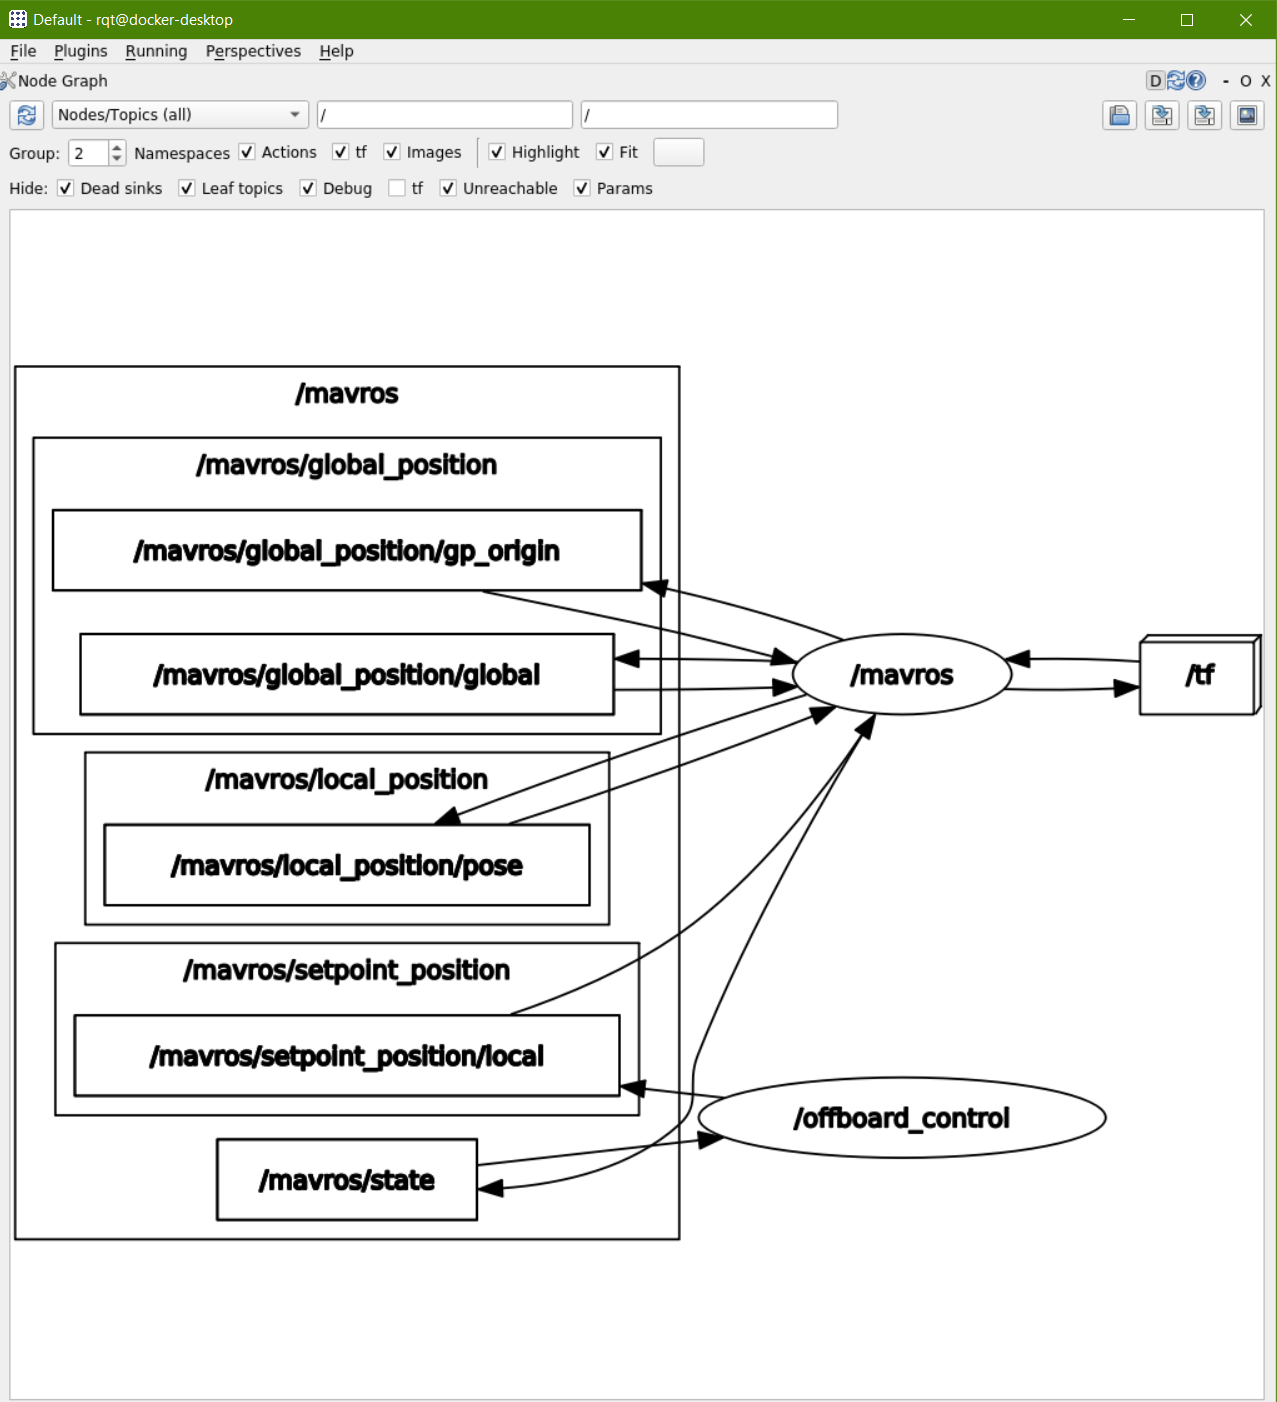
\includegraphics[width=0.5\textwidth]{images/rqt_graph.png} \label{fig:rqt_graph}}
    \subfloat[Topic-Explorer zeigt alle verbreiteten Nachrichten]{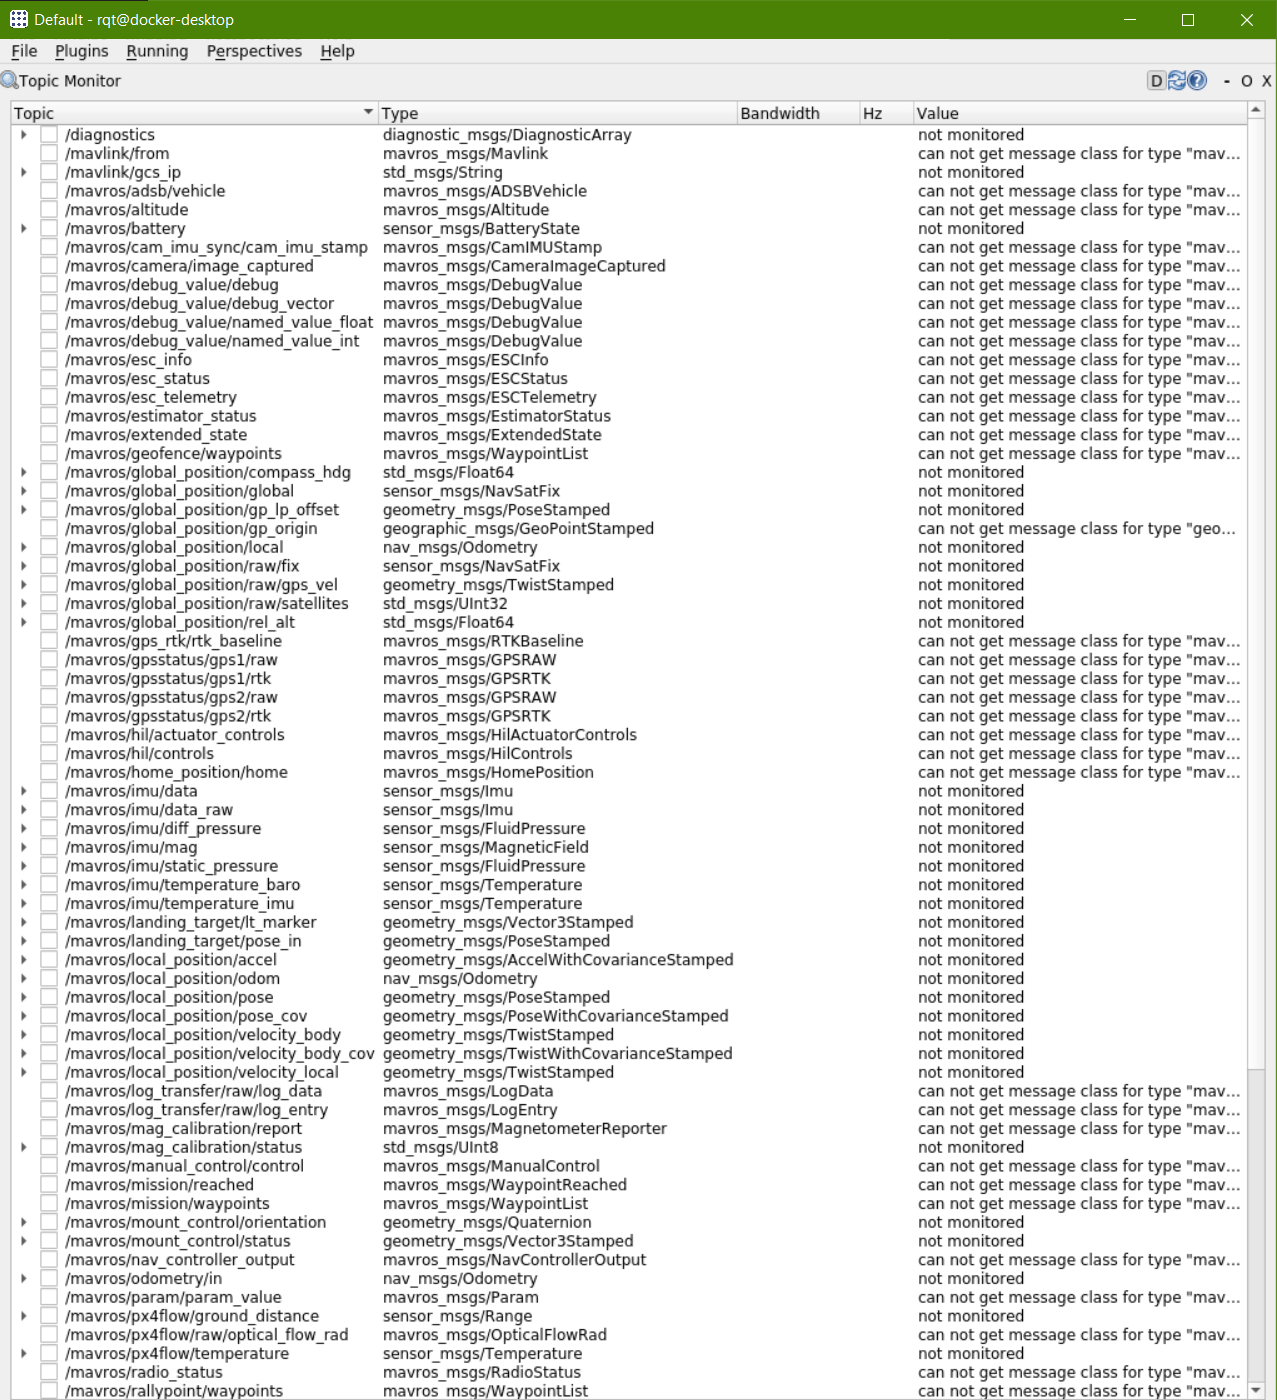
\includegraphics[width=0.5\textwidth]{images/rqt_topics.png} \label{fig:rqt_topic}}
    \caption{Graphische Anwendung \textit{rqt} aus ROS unter Windows}
    \label{fig:rqt}
\end{figure}

\subsubsection{mavros}
Zusätzliche Schritte, beschrieben in \cite{dronecodestiftungObstacleDetectionAvoidance2023} und \footnote{\url{https://docs.px4.io/main/en/ros/mavros_installation.html}\cite{dronecodestiftungPX4UserGuide}}, werden auf dem Image \enquote{noetic-perception-focal} ausgeführt um das Programm \enquote{mavros} zu installieren. Mit Start des Containers started auch \textit{mavros}. Dieses kann per Netzwerkzugriff auf den \gls{rpi} zugreifen. In der entsprechenden Konfigurationsdatei (\textit{Dockerfile}) wird die derzeitige IP-Adresse des \gls{rpi} und der Zugriff über TCP-Protokoll eingetragen. Spätere Anwendungen auf dem \gls{rpi} selbst müssen diese anpassen (es kann per UDP auf \textit{localhost} zugegriffen werden solange \textit{mavlink-routerd} läuft \textbf{oder} \textit{mavlink-routerd} wird komplett deaktiviert und \textit{mavros} erhält direkten Zugriff auf die Serielle Schnittstelle).

Wird \textit{mavros} im Container gestartet, erscheinen sogleich eine Vielzahl von Warnungen und Fehlern. Eine Warnung erscheint besonders häufig: \enquote{RTT too high for timesync}. Diese sagt aus, dass die Zeitverzögerung der Verbindung über Netzwerk zu groß sei. Eine Problemlösung ist diese Warnung abzustellen, beschrieben in \footnote{\url{https://discuss.ardupilot.org/t/rtt-too-high-for-timesync-with-sitl-mavros/38224}}. Die Prozedur wird auch für dieses Projekt angewandt, direkt während der Einrichtung von Docker. Die Folgen sind zum derzeitigen Zeitpunkt nicht abzuschätzen, wahrscheinlich wird eine Steuerung der Drohne über Netzwerk aufgrund von Verzögerungen nicht möglich sein.

\subsubsection{offboard\_control}
Die Beispielanwendung stammt aus der offiziellen Dokumentation \footnote{\url{https://docs.px4.io/main/en/ros/mavros_offboard_cpp.html}\cite{dronecodestiftungPX4UserGuide}}. Es wird die CPlusPlus-Variante genommen, da eine höhere Performance im Vergleich zu Python erwartet wurde. Um die virtuelle Drohne, ohne RC-Fernsteuerung fliegen zu lassen, muss die \gls{gcs} gestartet sein, und der Joystick-Modus aktiviert sein\footnote{\url{https://github.com/PX4/PX4-Autopilot/issues/18389}\cite{dronecodestiftungPX4UserGuide}}. Zusätzlich wurden die Timeouts \enquote{RC Loss Failsafe Trigger}, \enquote{Data Link Loss Failsafe Trigger} auf $10s$ erhöht, um eine Kommunikation über den \gls{rpi} zu ermöglichen.

Die Performance beim Start stellt jedoch das Programm insgesamt in Frage. Im Idealfall verharrt die Drohne in ruhiger Endlage wie in Bild \ref{fig:app_sim_ende} dargestellt. Teilweise fliegt sie aber schon beim Start quer durch die Gegend. Nebenbei wird durch die \gls{gcs} eine Kartenaufzeichnung erzeugt, die nicht der Bewegung im Simulator entspricht. Hindernisse in der Simulation werden nicht von der \gls{gcs} erkannt, stattdessen wird weiterhin eine Bewegung in entsprechende Richtung angenommen obwohl keine Bewegung stattfindet. Es ist deshalb möglich, dass die Drohne so in einem Hindernis stecken bleibt. Andernfalls bewegt sie sich irgendwann wieder an ihren Ausgangspunkt zurück.

Bild \ref{fig:rqt_graph} wurde aufgenommen als die Beispielanwendung lief. Es ist zu erkennen, dass das Programm Daten zum Status (\url{/mavros/state}) abfragt und Daten zum Positionsgeber (\url{/mavros/setpoint_position/local}) generiert. Diese Daten stehen im direkten Austausch zum \textit{mavros}-Knotenpunkt, der wiederum mit dem \gls{rpi} kommuniziert.
